\documentclass[preprint,12pt,authoryear]{elsarticle}

\usepackage{amsmath,amssymb,amsthm}
\usepackage{booktabs}
\usepackage{graphicx}
\usepackage{xcolor}
\usepackage[hidelinks]{hyperref}

\newtheorem{definition}{Definition}
\newtheorem{proposition}{Proposition}
\newtheorem{remark}{Remark}

\journal{Expert Systems with Applications}

\begin{document}

\begin{frontmatter}

\title{Fuzzy RFM formal concept analysis for customer segmentation:\\ boundary-aware, describable and stable segments}

% TODO: authors and affiliations
\author[a]{Author One\corref{cor1}}
\ead{author.one@example.edu}
\author[a]{Author Two}
\cortext[cor1]{Corresponding author.}
\affiliation[a]{organization={Department, University}, city={City}, country={Country}}

\begin{abstract}
Recency--frequency--monetary (RFM) segmentation with formal concept analysis (FCA) yields segments that are explicitly described and organised in a hierarchy, but its binary context assigns customers on either side of a quintile cut point to disjoint segments although they behave almost identically. We replace the binary RFM context with a fuzzy one and build segments from Bělohlávek fuzzy concepts. Three additions make this work in practice: a core-support threshold that removes the near-universal concepts which the Łukasiewicz residuum otherwise makes frequent, a greedy summary that selects a small set of concepts with a $(1-1/e)$ approximation guarantee, and a tie-aware membership for heavily tied frequencies. We prove that crisp RFM-FCA is a special case and that core support reduces to ordinary support on binary data. We replicate the crisp method of \citet{rungruang2024} and compare against it, against fuzzy memberships alone, log-RFM, and K-means, Gaussian mixture and fuzzy C-means clustering, on three retail datasets with rolling-origin out-of-sample evaluation and analysis plans committed before each analysis. Fuzzy RFM-FCA predicts next-period purchase and spend better than crisp RFM-FCA on all three datasets, with the result holding in 47 of 48 settings of a sensitivity analysis; it reaches more revenue in the top customer decile and gives the most robust and stable segments of all methods compared. It is not a better predictor than log-RFM and is roughly level with fuzzy C-means, but unlike clustering its segments are exactly described by short rules, and it represents the 69--74\,\% of customers who lie near a quintile boundary.
\end{abstract}

\begin{keyword}
Customer segmentation \sep RFM \sep Formal concept analysis \sep Fuzzy concept lattice \sep Fuzzy logic \sep Interpretability
\end{keyword}

\begin{highlights}
\item Fuzzy RFM context with Bělohlávek fuzzy concepts generalises crisp RFM-FCA.
\item A core-support threshold removes the near-universal concepts of the Łukasiewicz lattice.
\item Fuzzy RFM-FCA beats crisp RFM-FCA on three datasets and in 47 of 48 sensitivity settings.
\item It gives the most stable segments of all methods, with exact rule descriptions.
\item A greedy 10-concept summary with a $(1-1/e)$ guarantee makes it usable by marketers.
\end{highlights}


\end{frontmatter}

\section{Introduction}\label{sec:intro}

Recency, frequency and monetary value (RFM) remain the most widely used basis for behavioural customer segmentation because they are cheap to compute, easy to explain and strongly predictive of future purchasing \citep{hughes1994,fader2005}. In practice each dimension is scored by quintile and customers are grouped either by score combinations or by clustering the scores or raw values \citep{chen2012,wedel2000}. \citet{rungruang2024} proposed an alternative: treat the fifteen quintile indicators (R1--R5, F1--F5, M1--M5) as a binary formal context and read segments off its concept lattice \citep{ganter1999}. Unlike clusters, formal concepts are defined by their descriptions (an intent such as $\{R5, F5, M5\}$), are ordered in a hierarchy, and come with association rules between them, which makes them directly usable by marketers.

The binary context has a cost that \citet{rungruang2024} themselves identify as future work: a customer just below a quintile cut point and one just above it receive disjoint attributes although their behaviour is almost the same. We find that this is not a corner case: 69--74\,\% of customers in three retail datasets lie within 0.05 of a quintile cut point on at least one dimension (Section~\ref{sec:res-interp}). For these customers the crisp segment depends on a near-arbitrary line, and small data changes move them between segments.

This paper replaces the binary context with a fuzzy one and builds segments from fuzzy formal concepts \citep{belohlavek2002,belohlavek2004}. Taken naively, the extension fails: under the Łukasiewicz residuum every customer belongs at least half-way to any concept whose intent contains only partial terms, so thousands of uninformative concepts pass the usual support threshold, and models built on them overfit (Section~\ref{sec:res-dev}). We make the extension work and test it thoroughly. Our contributions are:

\begin{enumerate}
\item \textbf{Method.} A fuzzy RFM context on a percentile-rank scale whose 0.5-cut is exactly the crisp quintile context; a \emph{core-support} threshold for fuzzy concepts; a greedy \emph{summary} that selects a small set of concepts; and a \emph{tie-aware} membership for heavily tied frequencies.
\item \textbf{Theory.} Crisp RFM-FCA is a special case of the method; core support reduces to ordinary support on binary data and is anti-monotone; the Łukasiewicz floor explains why sigma-count support fails; and the summary objective is monotone submodular, so the greedy selection is within $1-1/e$ of optimal \citep{nemhauser1978}.
\item \textbf{Evidence.} A replication of \citet{rungruang2024} and a rolling-origin, out-of-sample comparison on three datasets against the crisp method, fuzzy memberships alone, log-RFM, and K-means, Gaussian-mixture and fuzzy C-means clustering, covering prediction, targeting value, robustness, stability, structural interpretability and sensitivity to every parameter fixed early. Analysis plans were committed to version control before each analysis, and the two later datasets serve as confirmation.
\end{enumerate}

The results are positive but bounded. Fuzzy RFM-FCA beats crisp RFM-FCA on every dataset and in 47 of 48 sensitivity settings, reaches more revenue in the most valuable customer decile and gives the most robust and stable segments of all methods. It is not a better predictor than a plain log-RFM model, it is roughly level with fuzzy C-means, and its full lattice has about four times as many segments as the crisp one, which the 10-concept summary addresses. We report these limits alongside the gains.

Section~\ref{sec:related} reviews related work, Section~\ref{sec:method} presents the method and its properties, Section~\ref{sec:design} the experimental design, Section~\ref{sec:results} the results, and Section~\ref{sec:discussion} their implications and limitations.

\section{Related work}\label{sec:related}

\paragraph{RFM segmentation} RFM summarises a customer's history by the time since the last purchase, the number of purchases and the amount spent \citep{hughes1994}. Its predictive value is well established: \citet{fader2005} show that RFM is a sufficient summary for customer-lifetime-value projection under standard purchase models, using the CDNOW data that we also use. Segmentation practice scores each dimension by quintile and either reads segments off score combinations or clusters customers, most often with K-means; \citet{chen2012} introduced the Online Retail data with an RFM/K-means case study, and K-means, hierarchical clustering and Gaussian mixtures remain the usual choices \citep{wedel2000}. Cluster-based segments, however, are described only by centroids and must be labelled after the fact, which is the gap FCA addresses.

\paragraph{Fuzzy RFM} Fuzziness has entered RFM work in two ways. \citet{carrasco2019} replace crisp RFM scores by 2-tuple fuzzy linguistic values before K-means segmentation, addressing the imprecision of ordinal scores. \citet{marindiaz2025} cluster RFM features with fuzzy C-means \citep{bezdek1981}, map them to a 2-tuple linguistic scale and add explainable-AI post-processing. In both, the segments are still clusters; fuzziness softens the inputs or the assignment, but segments do not carry explicit, exact descriptions or an order between them. Our work keeps FCA's explicit, ordered segments and makes the context itself fuzzy.

\paragraph{Formal concept analysis} FCA derives a lattice of concepts (extent, intent) from a binary object--attribute context \citep{ganter1999}. Surveys document its use for knowledge discovery, information retrieval and ontology engineering \citep{poelmans2013app,poelmans2013mod,singh2016}. Two practical issues recur: the number of concepts grows quickly, which motivates pruning by support, stability \citep{kuznetsov2007} or other indices, and binary contexts require discretising numeric data. Association rules between concepts are usually read along lattice covers \citep{luxenburger1991}. \citet{rungruang2024} applied FCA to quintile RFM scores and showed that the lattice gives an interpretable, hierarchical segmentation of Online Retail II customers, compared with K-means and hierarchical clustering by cluster-validity indices.

\paragraph{Fuzzy formal concept analysis} Fuzzy FCA generalises the binary incidence relation to degrees in a residuated lattice \citep{burusco1994,pollandt1997,belohlavek2002,belohlavek2004}; surveys review its variants and applications \citep{poelmans2014,alwersh2022}. A recurring issue, noted by \citet{alwersh2022}, is the much larger number of fuzzy concepts, which makes concept reduction necessary for applications. We address it with a scale-aware support notion (core support) and a summary with an approximation guarantee, and we show why the common sigma-count support is inadequate under the Łukasiewicz residuum.

\paragraph{Positioning} To our knowledge, fuzzy formal concepts have not been used for RFM segmentation, and RFM-FCA has not been evaluated out of sample, against clustering baselines on prediction, targeting and stability, or across several datasets. This paper does all three.

\section{Method}\label{sec:method}

\subsection{Crisp RFM-FCA}\label{sec:crisp}

Let $G$ be a set of customers. For each customer, recency $R$ (days since the last purchase), frequency $F$ (number of transaction lines) and monetary value $M$ (total spend) are computed at a cutoff date. Each dimension $d \in \{R,F,M\}$ is mapped to a mid-rank percentile $u_d(g) \in (0,1]$ among the fitted customers, oriented so that larger is better (recency is reversed). The crisp quintile score is $q_d(g) = \lceil 5\,u_d(g) \rceil$, and the crisp context is the binary relation $I \subseteq G \times M$ over the fifteen attributes $M = \{R1,\dots,R5,F1,\dots,F5,M1,\dots,M5\}$ with $(g, dk) \in I$ iff $q_d(g) = k$. Formal concepts are pairs $(A,B)$ with $A' = B$ and $B' = A$ under the usual derivation operators \citep{ganter1999}; a concept's \emph{support} is $|A|/|G|$, and \citet{rungruang2024} keep concepts with support at least $0.04$ as segments.

\subsection{Fuzzy RFM context}\label{sec:fuzzy-context}

\begin{definition}[Linguistic terms]
For $k=1,\dots,5$ let $c_k = (2k-1)/10$ be the quintile midpoints and $h = 0.2$ the half-width. The membership of rank $u$ in term $k$ is
\begin{equation}
\mu_k(u) = \max\!\left(0,\; 1 - \frac{|u - c_k|}{h}\right),
\end{equation}
with saturating shoulders $\mu_1(u) = 1$ for $u \le c_1$ and $\mu_5(u) = 1$ for $u \ge c_5$.
\end{definition}

The five terms form a Ruspini partition \citep{ruspini1969}: $\sum_k \mu_k(u) = 1$ and at most two adjacent terms are positive. A customer in the middle of a quintile band is fully in that term; a customer near a cut point is partly in the two neighbouring terms.

Memberships are rounded to the chain $L = \{0, \tfrac12, 1\}$ (``not'', ``partly'', ``fully''), which keeps the lattice finite and the segment descriptions readable. The fuzzy context is $\tilde I(g, dk) = \operatorname{round}_L \mu_k(u_d(g))$.

\subsection{Fuzzy concepts}\label{sec:fuzzy-concepts}

We use the fuzzy concept lattice of \citet{belohlavek2002,belohlavek2004} over the chain $L$ with a residuated implication $\to$; our primary choice is the Łukasiewicz residuum $a \to b = \min(1, 1-a+b)$, with the Gödel residuum ($a \to b = 1$ if $a \le b$, else $b$) as a check \citep{hajek1998}. For a fuzzy set of customers $A$ and of attributes $B$,
\begin{equation}
A^{\uparrow}(m) = \bigwedge_{g \in G} \bigl(A(g) \to \tilde I(g,m)\bigr), \qquad
B^{\downarrow}(g) = \bigwedge_{m \in M} \bigl(B(m) \to \tilde I(g,m)\bigr).
\end{equation}
A fuzzy concept is a pair $(A,B)$ with $A^{\uparrow} = B$ and $B^{\downarrow} = A$; $B^{\downarrow}(g)$ is customer $g$'s degree of membership in the concept. Since $A^{\uparrow}$ is the meet of the intents $\{a/g\}^{\uparrow} = a \to \tilde I(g,\cdot)$, the set of intents is the meet-closure of these generators together with the top element; we compute it by iterated pointwise minima over the distinct rows of $\tilde I$.

\begin{definition}[Core support]
The \emph{core extent} of a concept with intent $B$ is the crisp set $\{g : B^{\downarrow}(g) = 1\}$ and its \emph{core support} is $\mathrm{cs}(B) = |\{g : B^{\downarrow}(g) = 1\}| / |G|$. Concepts with $\mathrm{cs}(B) \ge 0.04$ (excluding the top concept) are the segments of \emph{fuzzy RFM-FCA}; customers are represented by their degrees $B^{\downarrow}(g)$ in these segments.
\end{definition}

Rules between segments are read along the covers of the order restricted to the segments, with confidence $\mathrm{cs}(B_2)/\mathrm{cs}(B_1)$ for $B_1 < B_2$, in the spirit of the Luxenburger basis \citep{luxenburger1991}.

\subsection{Properties}\label{sec:properties}

\begin{proposition}[Crisp RFM-FCA is a special case]\label{prop:special}
(i) If $u$ lies in the interior of quintile band $q$, then $\mu_q(u) > \tfrac12 > \mu_k(u)$ for all $k \ne q$; hence the 0.5-cut of the fuzzy context is the crisp quintile context. (ii) Over the two-element chain $\{0,1\}$ every residuated implication is classical implication, so the fuzzy concept lattice of a binary context equals its classical concept lattice, degrees are extent indicators, and core support equals support.
\end{proposition}
\begin{proof}
(i) Band $q$ is $((q-1)/5, q/5]$ with midpoint $c_q$; an interior point is less than $0.1$ from $c_q$ and more than $0.1$ from every other midpoint, so $\mu_q(u) > 1 - 0.1/0.2 = \tfrac12$ and $\mu_k(u) < \tfrac12$. (ii) On $\{0,1\}$ residuation forces $a \to b = 1$ iff $a \le b$, i.e.\ $0\to 0 = 0\to1 = 1\to1 = 1$ and $1 \to 0 = 0$; the operators $\uparrow,\downarrow$ then coincide with the derivation operators.
\end{proof}

\begin{proposition}[Core support]\label{prop:core}
For any residuated implication on a chain: (i) $B^{\downarrow}(g) = 1$ iff $B(m) \le \tilde I(g,m)$ for all $m$, so the core extent does not depend on the residuum; (ii) core support is anti-monotone: $B_1 \le B_2$ implies $\mathrm{cs}(B_2) \le \mathrm{cs}(B_1)$, so frequent intents form a down-set and can be mined level-wise; (iii) on a binary context core support equals ordinary support.
\end{proposition}
\begin{proof}
(i) In a residuated lattice $a \to b = 1$ iff $a \le b$, and a meet over a chain equals 1 iff every term does. (ii) If $B_1 \le B_2$ and $B_2(m) \le \tilde I(g,m)$ for all $m$, then $B_1(m) \le \tilde I(g,m)$. (iii) Follows from (i) and Proposition~\ref{prop:special}(ii).
\end{proof}

\begin{proposition}[Łukasiewicz floor]\label{prop:floor}
Under the Łukasiewicz residuum, $B^{\downarrow}(g) \ge 1 - \max_m B(m)$ for every customer. Consequently the sigma-count support $\sum_g B^{\downarrow}(g)/|G|$ of every intent whose degrees are all at most $\tfrac12$ is at least $\tfrac12$, and every such concept passes any support threshold $s \le \tfrac12$.
\end{proposition}
\begin{proof}
$a \to b = \min(1, 1-a+b) \ge 1-a$ for $b \ge 0$, and the meet over $m$ is at least $\min_m (1 - B(m)) = 1 - \max_m B(m)$.
\end{proof}

Proposition~\ref{prop:floor} explains the failure of the naive extension: on Online Retail II, 2,649 of 3,841 Łukasiewicz concepts reach a sigma-count support of $0.04$, dominated by intents such as $\{\tfrac12 F1, \tfrac12 F2, \tfrac12 M1, \tfrac12 M2\}$ with support around $0.52$. Core support is immune to the floor, and by Proposition~\ref{prop:core} it is the natural generalisation of the crisp threshold.

\subsection{Summary view}\label{sec:summary}

The full set of fuzzy segments is about four times larger than the crisp one (Section~\ref{sec:res-interp}). For communication we select $K$ segments. A customer's \emph{explained mass} given a set $S$ of segments is the largest intent size $w_c = \sum_m B_c(m)$ (a full term counts 1, a partial term $\tfrac12$) among segments in $S$ whose core contains the customer, or 0. The objective is
\begin{equation}
f(S) = \sum_{g \in G} \max_{c \in S} w_c \,\mathbf{1}\bigl[B_c^{\downarrow}(g) = 1\bigr], \qquad f(\emptyset) = 0,
\end{equation}
maximised greedily under $|S| = K$, with ties broken by larger core support. The selection uses no outcome variable.

\begin{proposition}[Greedy guarantee]\label{prop:greedy}
$f$ is non-negative, monotone and submodular; the greedy selection $S_K$ satisfies $f(S_K) \ge (1 - 1/e) \max_{|S| = K} f(S)$.
\end{proposition}
\begin{proof}
For each $g$, $S \mapsto \max_{c \in S} a_{gc}$ with $a_{gc} \ge 0$ is monotone and submodular (a facility-location term); sums of such functions inherit both properties. The bound is the classical result of \citet{nemhauser1978}.
\end{proof}

\subsection{Tie-aware memberships}\label{sec:ties}

When many customers share a value (e.g.\ the 52--65\,\% of CDNOW customers with a single purchase), the mid-rank places the whole block at one point and the fuzzy context cannot express that its members' quintile is ambiguous. A block of $n_t > 1$ tied customers occupies the rank interval $[l, r]$ of width $n_t/|G|$ centred on the mid-rank. The tie-aware membership is
\begin{equation}
\bar\mu_k = \frac{1}{r - l} \int_l^r \mu_k(u)\,\mathrm{d}u ,
\end{equation}
with $\bar\mu_k = \mu_k(u)$ for untied customers.

\begin{proposition}[Tie-aware memberships]\label{prop:ties}
$\bar\mu$ is the expected membership when the customer's position within the tied block is uniform; it is again a partition ($\sum_k \bar\mu_k = 1$), and it coincides with $\mu$ for untied values.
\end{proposition}
\begin{proof}
Linearity of the integral and $\sum_k \mu_k \equiv 1$.
\end{proof}

All five propositions are checked numerically in the accompanying test suite.

\section{Experimental design}\label{sec:design}

\subsection{Datasets}\label{sec:data}

\begin{itemize}
\item \textbf{Online Retail II} \citep{chen2019uci}: 1,067,371 transaction lines of a UK online gift wholesaler, December 2009 to December 2011; 5,878 customers after the base paper's cleaning. This is the base paper's dataset and was used for replication and method development.
\item \textbf{CDNOW} \citep{fader2005}: 69,659 purchases by 23,570 customers of an online music retailer who first bought in the first quarter of 1997, observed to June 1998. Between 52 and 65\,\% of customers have a single purchase at the cutoffs used.
\item \textbf{dunnhumby \emph{The Complete Journey}} \citep{dunnhumby}: 2,595,732 grocery basket lines of 2,500 households over 711 days; 92--93\,\% of households buy in any 90-day window.
\end{itemize}
Frequency counts transaction lines and monetary value is total spend, as in the base paper.

\subsection{Protocol}\label{sec:protocol}

We use rolling-origin evaluation \citep{tashman2000}: four cutoffs per dataset, three months apart; features use all transactions before a cutoff and targets the next 90 days. Targets are (a) whether a customer buys (ROC AUC, logistic regression) and (b) log spend (coefficient of determination $R^2$, ridge regression). Within each cutoff we use 5-fold cross-validation; the rank scale, lattice, concept selection and clustering are fitted on the training customers of each fold only, so nothing learned from test customers enters their features. Features are standardised; regularisation is either fixed ($C=1$, $\alpha=1$) or tuned by inner 3-fold cross-validation over $10^{-4},\dots,10^{2}$. Comparisons use a paired customer bootstrap (1,000 resamples within each cutoff) of the metric difference, pooled as the mean over cutoffs \citep{efron1993}, with Holm correction \citep{holm1979} within each pre-specified family.

\subsection{Representations compared}\label{sec:methods}

Each representation is fed to the same models (Table~\ref{tab:methods}). The two context representations isolate the effect of fuzzification; the lattice representations add the concept structure. Clustering baselines are fitted on standardised log-RFM: K-means, a full-covariance Gaussian mixture (GMM) and fuzzy C-means (FCM, fuzzifier 2, k-means++ seeding \citep{arthur2007,bezdek1981}), using one-hot membership, posterior probabilities and membership degrees respectively. The number of clusters is chosen in each training fold by the silhouette criterion over $k = 2,\dots,10$ as in the base paper \citep{rousseeuw1987}; as it selected $k = 2$ in all 60 training folds, we also report $k = 10$, which matches the size of the 10-concept summary.

\begin{table}[t]
\centering\small
\caption{Representations compared.}
\label{tab:methods}
\begin{tabular}{lll}
\toprule
Code & Description & Role \\
\midrule
C-ctx & 15 crisp quintile indicators & ablation \\
C-fca & crisp concepts with support $\ge 0.04$ \citep{rungruang2024} & base method \\
F-ctx & 15 fuzzy memberships & ablation \\
F-fca-core & fuzzy concepts with core support $\ge 0.04$ & proposed \\
F-sel$K$ / C-sel$K$ & $K$ fuzzy / crisp concepts, greedy summary & summary view \\
log-RFM & $\log(1+R), \log(1+F), \log(1+M)$ & benchmark \\
KM, GMM, FCM & clustering on log-RFM, silhouette $k$ and $k=10$ & baselines \\
\bottomrule
\end{tabular}
\end{table}

\subsection{Further measures}\label{sec:measures}

\textit{Targeting value}: the share of next-period revenue held by the top 10\,\% and 20\,\% of customers ranked by predicted spend, and the purchase-rate lift in the top 10\,\% and 20\,\% by predicted purchase probability. \textit{Robustness} and \textit{stability}: because concept sets and cluster labels are not directly comparable, we draw 20,000 random customer pairs, compute the cosine similarity of each pair's feature vectors under a reference fit and under a perturbed fit, and report the correlation of the two similarity vectors (1 = identical structure); perturbations are dropping 5\,\% of invoices (robustness) and bootstrap resampling of customers (stability), 20 replicates each. \textit{Structural interpretability}: description fidelity (F1 between satisfying a segment's R/F/M description and being a member; for clusters, the tightest quintile ranges holding 80\,\% of members), description length, number of segments and segments per customer.

\subsection{Pre-registration and staging}\label{sec:prereg}

The analysis plan and eleven addenda were committed to the project repository before the analysis each covers; deviations are listed in the repository. The method was developed on Online Retail II in two stages: the first specification (sigma-count support) failed and motivated core support (Section~\ref{sec:res-dev}). CDNOW and dunnhumby were then analysed once each with the method unchanged under confirmatory plans. Later analyses (clustering baselines, targeting, interpretability, summary, sensitivity) reuse the three datasets with plans committed before each; we label the tie-aware membership and the hybrid analysis as exploratory.

\section{Results}\label{sec:results}

\subsection{Replication of the base method}\label{sec:res-repl}

Our implementation of crisp RFM-FCA reproduces \citet{rungruang2024} on Online Retail II: 805,620 cleaned transaction lines, 5,878 customers and 208 formal concepts, as published. Over the 34 concept sizes printed in the paper the mean absolute difference is 0.8 customers (20 exact), and all 18 published association rules are recomputed with confidences within 0.01. Two reporting details had to be inferred: zero-price lines are kept (the published row count is reached only then), and recency is counted in calendar days.

\subsection{Method development and confirmation}\label{sec:res-dev}

The first fuzzy specification used sigma-count support. It was pre-registered on Online Retail II and failed: with fixed regularisation, the Łukasiewicz lattice (2,568--2,647 concepts per training fold) predicted worse than crisp RFM-FCA (AUC 0.733 vs 0.781, $R^2$ 0.173 vs 0.298), as Proposition~\ref{prop:floor} anticipates. Replacing it by core support reduces the segments to 208 on the full data. With fixed regularisation the core-filtered lattice was still slightly worse than the crisp one on Online Retail II (AUC $-0.007$), whereas with tuned regularisation it was better; tuned regularisation was therefore pre-specified for all later analyses.

The method was then tested unchanged on the two other datasets with seven pre-registered claims each. On CDNOW all seven replicated (Holm-adjusted $p = 0.005$ each): fuzzy memberships beat crisp scores, the fuzzy lattice beat the crisp lattice, the lattice added spend signal beyond the fuzzy memberships, and fuzzy representations changed less when transactions were dropped. On dunnhumby four replicated (memberships and lattice beating their crisp counterparts on both metrics) and three did not: the lattice predicted spend \emph{worse} than the fuzzy memberships ($R^2$ $-0.008$), and neither robustness claim held. These two findings are therefore not general, and we do not claim them.

\subsection{Prediction}\label{sec:res-pred}

\begin{table}[t]
\centering\small
\caption{Out-of-sample prediction of the next 90 days (means over four cutoffs; regularisation tuned by inner cross-validation). Best value per column in bold.}
\label{tab:prediction}
\begin{tabular}{lcccccc}
\toprule
 & \multicolumn{3}{c}{ROC AUC (purchase)} & \multicolumn{3}{c}{$R^2$ (log spend)} \\
\cmidrule(lr){2-4}\cmidrule(lr){5-7}
Representation & Retail II & CDNOW & dunnhumby & Retail II & CDNOW & dunnhumby \\
\midrule
Crisp scores (C-ctx) & 0.782 & 0.784 & 0.869 & 0.296 & 0.209 & 0.511 \\
Crisp RFM-FCA (C-fca) & 0.780 & 0.784 & 0.855 & 0.299 & 0.222 & 0.508 \\
Fuzzy memberships (F-ctx) & \textbf{0.787} & \textbf{0.789} & 0.877 & 0.304 & 0.219 & \textbf{0.525} \\
Fuzzy RFM-FCA (F-fca-core) & 0.786 & 0.788 & 0.865 & \textbf{0.308} & 0.235 & 0.517 \\
log-RFM & 0.786 & 0.788 & \textbf{0.887} & 0.293 & \textbf{0.241} & 0.517 \\
K-means, $k{=}10$ & 0.764 & 0.777 & 0.828 & 0.289 & 0.236 & 0.498 \\
GMM, $k{=}10$ & 0.770 & 0.778 & 0.875 & 0.260 & 0.232 & 0.453 \\
FCM, $k{=}10$ & 0.783 & 0.786 & 0.860 & 0.290 & 0.239 & 0.511 \\
\bottomrule
\end{tabular}
\end{table}

\begin{table}[t]
\centering\small
\caption{Paired differences (first minus second representation), tuned regularisation, pooled over four cutoffs. $^{*}$: 95\,\% customer-bootstrap interval excludes zero.}
\label{tab:comparisons}
\begin{tabular}{lcccccc}
\toprule
 & \multicolumn{3}{c}{$\Delta$ AUC} & \multicolumn{3}{c}{$\Delta R^2$} \\
\cmidrule(lr){2-4}\cmidrule(lr){5-7}
Comparison & Retail II & CDNOW & dunnhumby & Retail II & CDNOW & dunnhumby \\
\midrule
Fuzzification (memberships) & +0.0048$^{*}$ & +0.0048$^{*}$ & +0.0076$^{*}$ & +0.0080$^{*}$ & +0.0099$^{*}$ & +0.0141$^{*}$ \\
Fuzzy vs crisp RFM-FCA & +0.0063$^{*}$ & +0.0040$^{*}$ & +0.0098$^{*}$ & +0.0089$^{*}$ & +0.0124$^{*}$ & +0.0089$^{*}$ \\
Lattice beyond memberships & -0.0008 & -0.0007 & -0.0117$^{*}$ & +0.0044$^{*}$ & +0.0154$^{*}$ & -0.0082$^{*}$ \\
vs K-means, $k{=}10$ & +0.0220$^{*}$ & +0.0111$^{*}$ & +0.0372$^{*}$ & +0.0189$^{*}$ & -0.0017 & +0.0186$^{*}$ \\
vs GMM, $k{=}10$ & +0.0163$^{*}$ & +0.0102$^{*}$ & -0.0101$^{*}$ & +0.0487$^{*}$ & +0.0024 & +0.0634$^{*}$ \\
vs FCM, $k{=}10$ & +0.0029$^{*}$ & +0.0021$^{*}$ & +0.0052 & +0.0180$^{*}$ & -0.0047$^{*}$ & +0.0058 \\
\bottomrule
\end{tabular}
\end{table}


Table~\ref{tab:prediction} gives the out-of-sample accuracy of all representations and Table~\ref{tab:comparisons} the key paired differences. Three results hold on all three datasets. First, fuzzification helps: fuzzy memberships beat crisp quintile scores by 0.005--0.008 AUC and 0.008--0.014 $R^2$. Second, fuzzy RFM-FCA beats crisp RFM-FCA by 0.004--0.010 AUC and 0.009--0.012 $R^2$. Third, it beats K-means with ten clusters in five of six cells and the Gaussian mixture in four. Against fuzzy C-means with ten clusters it is roughly level (slightly better on Online Retail II, mixed on CDNOW, no significant difference on dunnhumby). With the silhouette-chosen $k = 2$ every clustering baseline is far behind (by 0.018--0.181 AUC), which mostly shows that two segments are too coarse.

No segmentation is a better predictor than log-RFM, which keeps the exact values that segments compress: it is best on dunnhumby AUC and CDNOW $R^2$, while fuzzy RFM-FCA is best on Online Retail II $R^2$ and the fuzzy memberships on dunnhumby $R^2$. An exploratory hybrid confirms that segment features carry information beyond the exact values for spend: adding fuzzy concept degrees to log-RFM raises $R^2$ by 0.020 (Online Retail II) and 0.015 (CDNOW), although not purchase AUC, and plain fuzzy memberships do as well in that role.

\subsection{Targeting value}\label{sec:res-target}

\begin{table}[t]
\centering\small
\caption{Share of next-90-day revenue (\%) held by the top 10\,\% and 20\,\% of customers ranked by predicted spend (means over four cutoffs).}
\label{tab:targeting}
\begin{tabular}{lcccccc}
\toprule
 & \multicolumn{3}{c}{Top 10\,\%} & \multicolumn{3}{c}{Top 20\,\%} \\
\cmidrule(lr){2-4}\cmidrule(lr){5-7}
Representation & Retail II & CDNOW & dunnhumby & Retail II & CDNOW & dunnhumby \\
\midrule
Crisp RFM-FCA (C-fca) & 52.6 & 52.6 & 28.3 & 71.6 & 70.6 & 50.1 \\
Fuzzy RFM-FCA (F-fca-core) & 55.4 & 53.5 & 30.5 & 71.8 & 70.4 & 50.7 \\
Fuzzy memberships (F-ctx) & 55.6 & 52.8 & 30.6 & 73.4 & 70.1 & 50.9 \\
log-RFM & 58.0 & 52.8 & 31.2 & 72.3 & 69.9 & 50.0 \\
K-means, $k{=}10$ & 54.1 & 51.6 & 28.6 & 70.3 & 68.7 & 48.3 \\
GMM, $k{=}10$ & 51.2 & 51.2 & 21.7 & 70.1 & 68.0 & 38.7 \\
FCM, $k{=}10$ & 36.2 & 53.8 & 26.8 & 71.2 & 70.2 & 49.5 \\
\bottomrule
\end{tabular}
\end{table}


\begin{figure}[t]
\centering
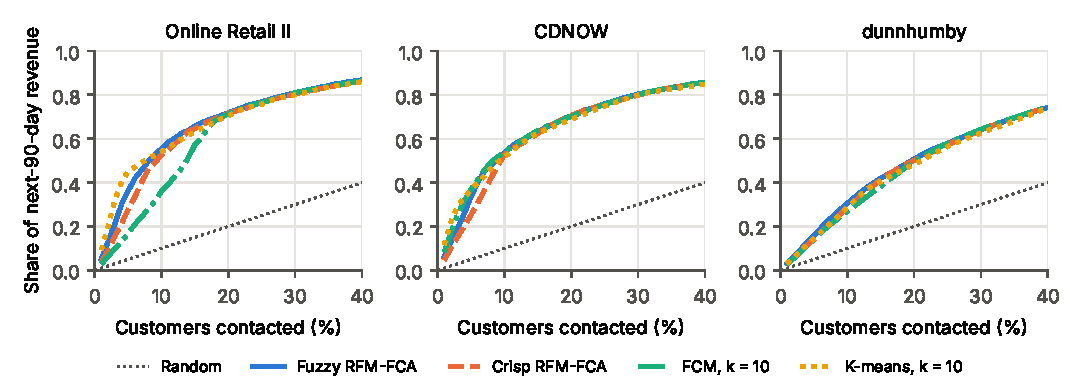
\includegraphics[width=\textwidth]{figures/gain_curves.pdf}
\caption{Cumulative share of next-90-day revenue against the share of customers contacted, ranked by predicted spend (means over four cutoffs).}
\label{fig:gain}
\end{figure}

Table~\ref{tab:targeting} and Figure~\ref{fig:gain} translate predictions into campaign terms. Contacting the top 10\,\% of customers ranked by fuzzy RFM-FCA reaches 0.9--2.9 percentage points more of next-period revenue than ranking by crisp RFM-FCA on every dataset ($p \le 0.01$), the decile where crisp quintile boundaries lump very different spenders together. Fuzzy RFM-FCA reaches more revenue than K-means and GMM at both depths on all datasets; fuzzy C-means is mostly level but fails on the Online Retail II top decile (36.2\,\% vs 55.4\,\%). Of the twelve pre-registered tests at 20\,\% depth (against crisp RFM-FCA and fuzzy C-means, revenue and lift), three are significant, all in favour of fuzzy RFM-FCA. Purchase lift on dunnhumby cannot exceed about 1.08 because almost all households buy, and is uninformative there.

\subsection{Robustness and stability}\label{sec:res-struct}

\begin{table}[t]
\centering\small
\caption{Structural agreement (correlation of customer-pair similarities between a reference fit and a perturbed fit; 1 = identical), mean over 20 replicates. Robustness: 5\,\% of invoices dropped. Stability: bootstrap resample of customers.}
\label{tab:structure}
\begin{tabular}{lcccccc}
\toprule
 & \multicolumn{3}{c}{Robustness} & \multicolumn{3}{c}{Stability} \\
\cmidrule(lr){2-4}\cmidrule(lr){5-7}
Representation & Retail II & CDNOW & dunnhumby & Retail II & CDNOW & dunnhumby \\
\midrule
Crisp RFM-FCA (C-fca) & 0.886 & 0.936 & 0.928 & 0.957 & 0.987 & 0.936 \\
Fuzzy RFM-FCA (F-fca-core) & 0.958 & 0.955 & 0.948 & 0.986 & 0.993 & 0.972 \\
K-means, $k{=}10$ & 0.760 & 0.907 & 0.650 & 0.683 & 0.937 & 0.692 \\
GMM, $k{=}10$ & 0.858 & 0.816 & 0.878 & 0.818 & 0.904 & 0.843 \\
FCM, $k{=}10$ & 0.913 & 0.929 & 0.942 & 0.944 & 0.966 & 0.914 \\
\bottomrule
\end{tabular}
\end{table}


At comparable granularity (Table~\ref{tab:structure}) fuzzy RFM-FCA has the highest mean robustness and stability of all representations on all three datasets. It beats crisp RFM-FCA in 20 of 20 robustness replicates on every dataset, and K-means and GMM in essentially every replicate. Against fuzzy C-means the margin is small and each method wins some replicates, but the worst case of fuzzy RFM-FCA is better in all six dataset--measure cells.

\subsection{Interpretability and the summary view}\label{sec:res-interp}

\begin{table}[t]
\centering\small
\caption{Structural interpretability proxies on the full data (Retail II / CDNOW / dunnhumby). Fidelity: F1 between ``satisfies the segment's R/F/M description'' and ``is a member''. Conditions: constrained dimensions per description.}
\label{tab:interpretability}
\begin{tabular}{lcccc}
\toprule
Representation & Segments & Fidelity (F1) & Conditions & Segments per customer \\
\midrule
Crisp RFM-FCA (C-fca) & 51 / 54 / 49 & 1.00 / 1.00 / 1.00 & 1.5 / 1.6 / 1.5 & 5.3 / 6.2 / 5.5 \\
Fuzzy RFM-FCA (F-fca-core) & 208 / 238 / 215 & 1.00 / 1.00 / 1.00 & 1.8 / 1.9 / 1.8 & 19.5 / 24.0 / 20.9 \\
K-means, $k{=}10$ & 10 / 10 / 10 & 0.68 / 0.74 / 0.74 & 3.0 / 3.0 / 3.0 & 1.0 / 1.0 / 1.0 \\
GMM, $k{=}10$ & 10 / 10 / 10 & 0.53 / 0.80 / 0.67 & 3.0 / 3.0 / 3.0 & 1.0 / 1.0 / 1.0 \\
FCM, $k{=}10$ & 10 / 10 / 10 & 0.66 / 0.71 / 0.73 & 3.0 / 3.0 / 3.0 & 1.0 / 1.0 / 1.0 \\
\bottomrule
\end{tabular}
\end{table}


Table~\ref{tab:interpretability} compares structural proxies. FCA segments are exactly described by their intents (fidelity 1 by construction) in fewer than two conditions on average, whereas the tightest R/F/M description of a cluster disagrees with its membership for 20--47\,\% of customers and constrains all three dimensions. Fuzzy RFM-FCA additionally represents the 74\,\%, 69\,\% and 73\,\% of customers who lie within 0.05 of a quintile cut point on at least one dimension. Its costs are about four times as many segments as crisp FCA (each customer belongs to about 20) and a rule set whose mean confidence is slightly \emph{lower} than the crisp one (0.71 vs 0.73, 0.81 vs 0.84, 0.79 vs 0.81), although individual rules become sharper: on Online Retail II, the crisp rule $\{R5, M5\} \Rightarrow \{R5, F5, M5\}$ has confidence 0.81, while its boundary-aware counterpart $\{R5, M5\} \Rightarrow \{R5, \tfrac12 F5, M5\}$ has 0.92.

\begin{table}[t]
\centering\small
\caption{The 10-concept fuzzy summary of Online Retail II (greedy description-coverage selection, full data). $\tfrac12$X: partly in term X.}
\label{tab:summaryview}
\begin{tabular}{rlrr}
\toprule
\# & Intent & Customers fully in (\%) & Share of spend (\%) \\
\midrule
1 & \{F5, M5\} & 10.3 & 55.3 \\
2 & \{F1, M1\} & 9.9 & 0.4 \\
3 & \{$\tfrac12$F2, $\tfrac12$M2\} & 18.9 & 2.7 \\
4 & \{$\tfrac12$F4, $\tfrac12$M4\} & 18.8 & 13.0 \\
5 & \{$\tfrac12$F3, $\tfrac12$M3\} & 17.9 & 5.6 \\
6 & \{$\tfrac12$F2, M1\} & 4.6 & 0.2 \\
7 & \{F5, $\tfrac12$M4\} & 4.5 & 3.6 \\
8 & \{$\tfrac12$F4, $\tfrac12$F5, $\tfrac12$M5\} & 6.3 & 11.8 \\
9 & \{$\tfrac12$F1, $\tfrac12$M1, $\tfrac12$M2\} & 6.2 & 0.6 \\
10 & \{R5, F5, M5\} & 4.8 & 36.9 \\
\bottomrule
\end{tabular}
\end{table}


The greedy summary addresses the segment count. Table~\ref{tab:summaryview} shows the ten fuzzy segments selected on Online Retail II; they include the high-value groups $\{F5, M5\}$ (10.3\,\% of customers, 55.3\,\% of spend) and $\{R5, F5, M5\}$ (4.8\,\%, 36.9\,\%) and band-straddling groups such as $\{\tfrac12 F4, \tfrac12 F5, \tfrac12 M5\}$. Each customer falls into one or two segments, described by about two conditions. As predictors, the 10-concept fuzzy summary beats the 10-concept crisp summary on all three datasets (AUC $+0.026$, $+0.005$, $+0.016$; $R^2$ $+0.033$, $+0.004$, $+0.011$; Holm $p \le 0.008$) and is far more robust and stable (the crisp summary collapses to a robustness of 0.57 on Online Retail II). Compression has a price: the summary predicts worse than the full lattice and than fuzzy C-means with ten clusters (AUC $-0.005$ to $-0.047$).

\subsection{Sensitivity}\label{sec:res-sens}

\begin{table}[t]
\centering\small
\caption{Sensitivity analysis: number of setting $\times$ dataset $\times$ metric cells in which the fuzzy variant is significantly better (95\,\% interval above zero) and significantly worse. Settings: support 0.02/0.04/0.06, membership half-width 0.15/0.20/0.25, horizon 60/90/180 days.}
\label{tab:sensitivity}
\begin{tabular}{lcc}
\toprule
Comparison & Fuzzy significantly better & Significantly worse \\
\midrule
Fuzzy vs crisp RFM-FCA & 47 / 48 & 0 \\
Fuzzy vs crisp memberships & 29 / 30 & 1 \\
Fuzzy vs crisp summary ($K = 5, 10, 20, 30$) & 18 / 24 & 1 \\
\bottomrule
\end{tabular}
\end{table}


\begin{figure}[t]
\centering
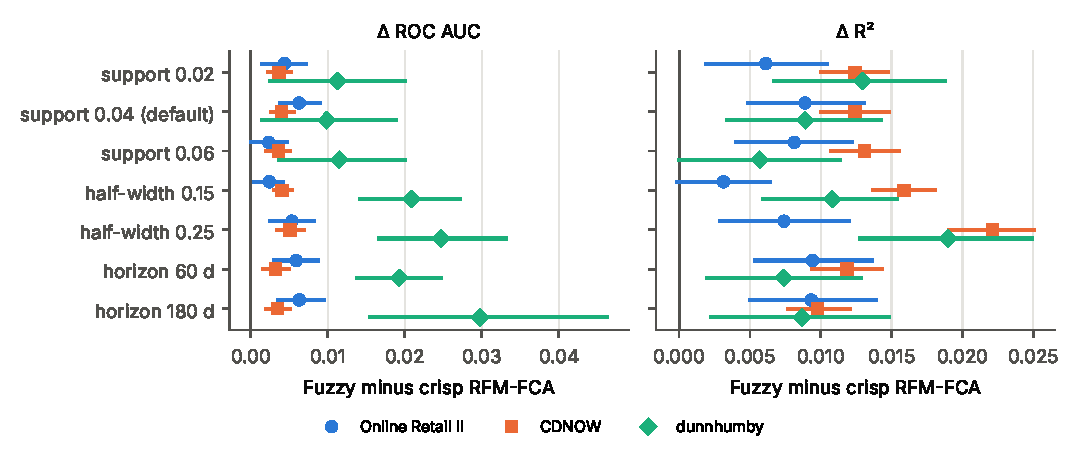
\includegraphics[width=\textwidth]{figures/sensitivity.pdf}
\caption{Difference between fuzzy and crisp RFM-FCA under one-at-a-time parameter changes, with 95\,\% customer-bootstrap intervals.}
\label{fig:sens}
\end{figure}

Every parameter fixed early was varied on all three datasets: the support threshold (0.02, 0.04, 0.06, which changes the number of fuzzy segments from about 140 to about 500), the membership half-width (0.15, 0.20, 0.25) and the horizon (60, 90, 180 days). Fuzzy RFM-FCA is significantly better than crisp RFM-FCA in 47 of 48 cells and never worse (Table~\ref{tab:sensitivity}, Figure~\ref{fig:sens}); the fuzzy-membership result holds in 29 of 30, with one reversal at the narrowest width. For the summary, $K = 10$ is the only size that beats the crisp summary in all six cells.

\subsection{Tie-aware memberships (exploratory)}\label{sec:res-ties}

On CDNOW, the mid-rank places all 11,840 one-time buyers in a single term, and 41 of the fuzzy rules merely restate this tie (e.g.\ $\{\tfrac12 F2\} \Rightarrow \{F2\}$ with confidence 1). The tie-aware membership spreads them over F1--F3, removes all 41 such rules and raises the bootstrap stability of the segment set from 0.908 (worst case 0.524) to 0.963 (worst case 0.920), with unchanged predictions. On the other two datasets it changes at most 0.8\,\% of customers. This was designed after seeing the CDNOW results and is exploratory.

\section{Discussion}\label{sec:discussion}

\subsection{What fuzzification buys}

The most consistent finding is that representing customers near quintile boundaries by partial memberships improves on hard quintiles, both as raw attributes and as concept lattices, on three datasets and across every parameter setting we tried. The mechanism is simple: about 70\,\% of customers lie near some cut point, and the crisp context separates customers who behave alike while merging customers who do not. The gain is concentrated where it matters commercially, in the top decile of spenders. Robustness and stability point the same way: fuzzy RFM-FCA gives the most stable segment structure of all representations compared, including the crisp lattice and every clustering baseline at comparable granularity.

\subsection{What it does not buy}

Three limits are equally consistent. First, segments are a compression: a plain log-RFM model is at least as accurate for prediction and targeting, so fuzzy RFM-FCA should not be sold as a forecasting engine. Second, most of the predictive gain comes from fuzzifying the context rather than from the lattice; the lattice added spend signal beyond the fuzzy memberships on two datasets and lost it on the third. Third, the full fuzzy lattice has about four times as many segments as the crisp one, and its rules are not more confident on average. Against fuzzy C-means, the natural fuzzy alternative, accuracy is roughly level.

\subsection{Practical recommendation}

These results suggest a two-level use. The full fuzzy lattice is the modelling representation: it predicts and targets better than crisp RFM-FCA and K-means and is the most stable. The 10-concept summary is the communication layer: ten named segments, each defined by about two conditions such as ``fully frequent and high-spending, at least partly very recent'', with the greedy guarantee of Proposition~\ref{prop:greedy}. If only predictions from unnamed groups are needed, fuzzy C-means or log-RFM are simpler and as good. What fuzzy RFM-FCA offers that neither does is segments that are exactly described, ordered, linked by rules and aware of boundary customers.

\subsection{Limitations}

\begin{itemize}
\item Effect sizes over crisp RFM-FCA are small (0.004--0.010 AUC, 0.009--0.012 $R^2$), and on smaller datasets the fuzzy lattice needs tuned regularisation.
\item Interpretability was assessed with structural proxies only; a study with marketers is needed to confirm that the segments are more useful in practice.
\item The method was developed on Online Retail II and confirmed on two further datasets; the later analyses reuse the same three datasets, and the tie-aware membership and the hybrid analysis are exploratory.
\item Only one family of memberships (triangular on the rank scale) and a three-level truth scale were studied; a five-level scale was computationally infeasible with our closure algorithm.
\item All datasets are retail; other sectors and contractual settings remain untested.
\end{itemize}

\section{Conclusion}\label{sec:conclusion}

We extended RFM segmentation with formal concept analysis from a binary to a fuzzy context, as proposed by \citet{rungruang2024}, and made the extension work with a core-support threshold, a greedy summary with an approximation guarantee and tie-aware memberships. Crisp RFM-FCA is a special case of the method. In a replication and a rolling-origin evaluation on three datasets with pre-registered analyses, fuzzy RFM-FCA beat crisp RFM-FCA on prediction, top-decile targeting, robustness and stability, a result that held in 47 of 48 sensitivity settings; it beat K-means and mostly the Gaussian mixture and was roughly level with fuzzy C-means, while providing segments with exact rule descriptions. It is not a better predictor than log-RFM, and its full lattice needs a summary to be usable. Future work should test the segments with marketers, extend the truth scale and membership families, and study non-retail settings.


\section*{Data and code availability}
Online Retail II \citep{chen2019uci} and CDNOW \citep{fader2005} are publicly available; dunnhumby \emph{The Complete Journey} \citep{dunnhumby} is available from its provider under its terms of use. All code, analysis plans (with commit history) and aggregate results are available at \url{https://github.com/nandana-das/rfm-fuzzy}.

\section*{Declaration of competing interest}
% TODO: confirm
The authors declare no competing interests.

\bibliographystyle{elsarticle-harv}
\bibliography{refs}

\end{document}
